% Chapter 1

\chapter{Gesture recognition in the cultural heritage scenario}

\lhead{Chapter 4. \emph{Hand gesture recognition}} % This is for the header on each page - perhaps a shortened title

%----------------------------------------------------------------------------------------
\section{Motivation}
In recent years the interest in cultural heritage has reborn, and the cultural market is becoming a cornerstone in many national economic strategies. In the United States, a recent report of the Office of Travel and Tourism Industries claims that 51\% of the 40 million Americans traveling abroad visit historical places; almost one third visit cultural heritage sites; and one quarter go to an art gallery or museum \cite{tourismintelligence}. The same interest is found in Europe, where the importance of the cultural sector is widely acknowledged, South Asia and North Africa. The latest annual research from World Travel and Tourism Council shows that travel and tourism's total contribution to total GDP grew by 3.0\% in 2013, faster than overall economic growth for the third consecutive year \cite{econotravel}.

Consequently, to deal with an increasing percentage of ``digital native'' tourists, a big effort is under way to propose new interfaces for interacting with the cultural heritage.
 In this direction goes the solution ``SmartMuseum'' proposed by Kuusik \etal \cite{kuusik2009smartmuseum}: by the means of PDAs and RFIDs, a visitor can gather information about what the museum displays, building a customized visit based on his or her interests inserted, prior to the visit, on their website. This project brought an interesting novelty when first released, but it has some limitations. First, being tied to RFIDs does not allow reconfiguring the museum without rethinking the entire structure of the exhibition. Furthermore, researches demonstrated how the use of mobile devices on the long term decreases the quality of the visit due to their users paying more attention to the tool rather than to the work of art itself.

In 2007 Kuflik \etal \cite{kuflik2011visitor} proposed a system to customize visitors experiences in museums using software capable of learning their interests based on the answers to a questionnaire that they compiled before the visit. Similarly to SmartMuseum, one of the main shortcomings of this system is the need to stop the visitor and force him into doing something that he/she might not be willing to do.
An interesting attempt to user profiling with wearable sensors was the Museum Wearable \cite{sparacino2002museum}, a wearable computer which orchestrates an audiovisual narration as a function of the visitors' interests gathered from his/her physical path in the museum. However this prototype does not use any computer vision algorithm for understanding the surrounding environment. For instance the estimation of the visitor location is based again on infrared sensors distributed in the museum space.

Museums and cultural sites still lack of an instrument that provides entertainment, instructions and visit customization in an effective natural way. Too often visitors struggle to find the description of the artwork they are looking at and when they finds it, its detail level could be too high or too low for their interests. Moreover, frequently the organization of the exhibition does not reflect the visitors' interests leading them to a pre-ordered path which cultural depth could not be appropriate.

To overcome these limitations, we present a solution to enhance visitors' experiences based on a new emerging technology, namely \textit{ego-vision} \cite{kanade2012}. Ego-vision features glass-mounted wearable cameras able to see what the visitor sees and perceiving the surrounding environment as he does. We developed a wearable vision device for museum environments, able to replace the traditional self-service guides and overcoming their limitations and allowing for a more interactive museum experience to all visitors. The aim of our device is to stimulate the visitors to interact with the artwork, reinforcing their real experience, by letting visitors to replicate the gestures (e.g. point out to the part of the painting they're interested in) and behaviors that they would use to ask a guide something about the artwork.

In this work, we provide algorithms that perform gesture analysis to recognize user interaction with artworks, and artwork recognition to achieve content-awareness.
The proposed solution is based on scalable and distributed wearable devices capable of communicating with each other and with a central server and hence does not require fixed cameras.
In particular the connection with the central server allows our wearable devices to grab gestures of past visitors for improving gesture analysis accuracy, to get information and specific content of the observed artwork through the automatic recognition module, and to share visitor's feelings and photos on social networks. 

The proposed gesture recognition algorithm is compared to the current state of the art on benchmark datasets showing superior performance, and is tested in real and virtual museum environments. We further demonstrate that our gesture recognition approach can achieve acceptable accuracy results even with a few training samples performed by the visitor, and can benefit from distributed training in which gestures performed by other visitors are exploited. Finally, we present a performance evaluation of our algorithms on an ARM Cortex A15 multicore platform for mobile/wearable devices.


\section{Proposed Method}
To our knowledge, the study of gesture recognition in the ego-centric paradigm has not yet been addressed. Even though not related to ego-vision domain, several approaches to gesture and human action recognition have been proposed. Sanin \etal \cite{sanin2013spatio} developed a new and more effective spatio-temporal covariance descriptor to classify gestures in conjunction with a boost classifier. Lui \etal \cite{lui2010action, lui2011tangent} used tensors and tangent bundle on Grassmann manifolds to classify human actions and hand gestures. Kim \etal \cite{kim2009canonical} extended Canonical Correlation Analysis to measure video-to-video similarity to represent and detect actions in video. However, all these approaches are not appropriate for the ego-centric perspective, as they do not take into account any of the specific characteristics of this domain, such as fast camera motion and background cluttering.
\begin{figure}
\centering
\subfigure{
                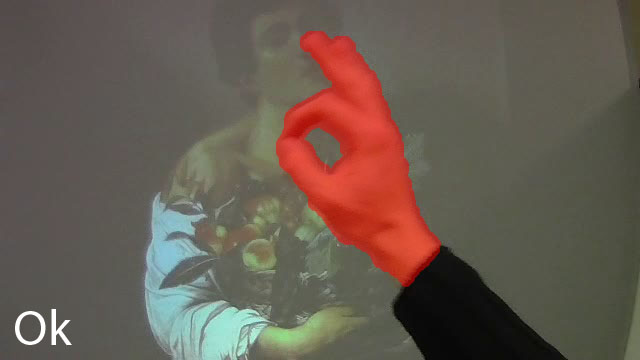
\includegraphics[width=0.23\textwidth]{Figures/ok_7141_7164_text16.jpg}
                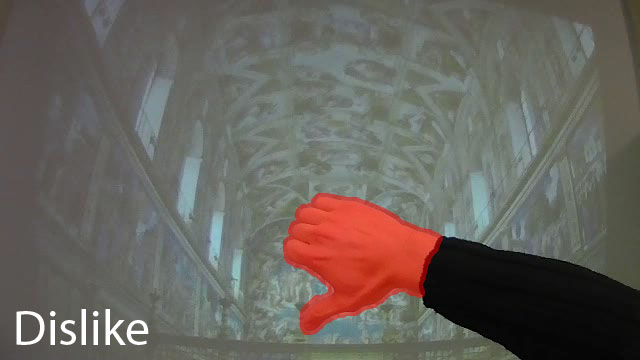
\includegraphics[width=0.23\textwidth]{Figures/dislike_3941_3969_text16.jpg}
} \\
\subfigure{
	    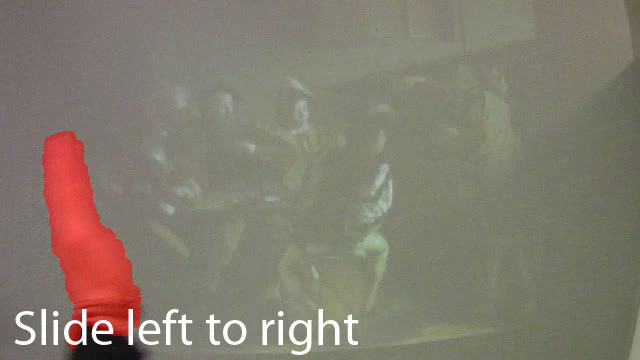
\includegraphics[width=0.23\textwidth]{Figures/slide_2_7438_7451_text5.jpg}
                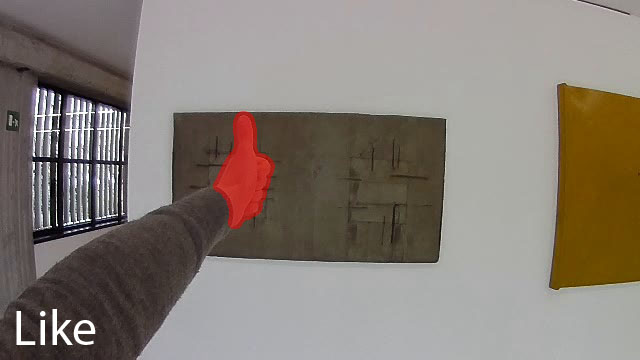
\includegraphics[width=0.23\textwidth]{Figures/like_7038_7080_text23.jpg}
} \\
\subfigure{
                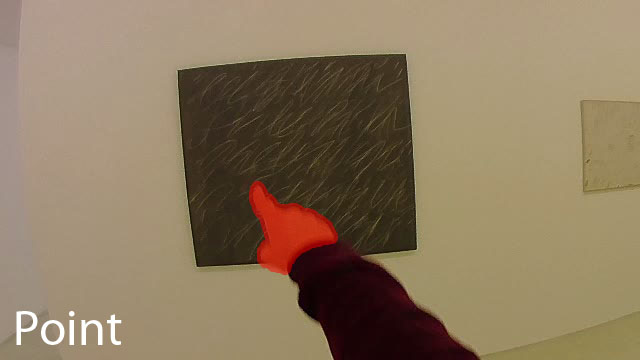
\includegraphics[width=0.23\textwidth]{Figures/point_15476_15505_text5.jpg}
                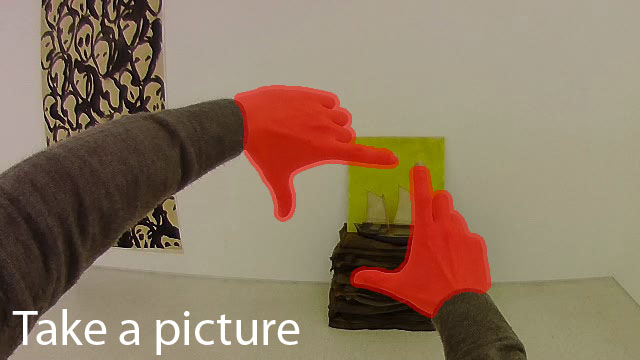
\includegraphics[width=0.23\textwidth]{Figures/take_a_picture_18622_18673_text37.jpg}
} \\
\caption{Natural interaction with artworks: visitors can get specific content or share information about the observed artwork through simple gestures. Hand segmentation results are highlighted in red and detected gestures are reported in the bottom part of each frame.}
\label{sample}
\end{figure}

\begin{figure}
\centering
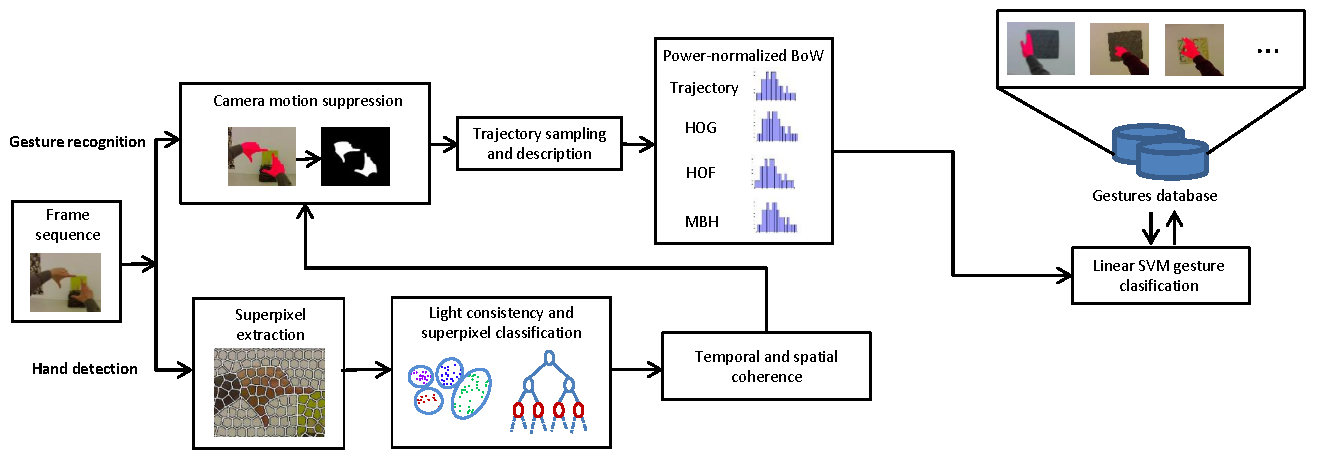
\includegraphics[width=\linewidth]{Figures/schema.pdf}
\caption{Outline of the proposed Gesture Recognition method.}
\label{schema}
\end{figure}
Gesture recognition systems should recognize both static and dynamic hand movements. Therefore, we propose to describe each gesture as a collection of dense trajectories extracted around hand regions. Feature points are sampled inside and around the user's hands and tracked during the gesture; then several descriptors are computed inside a spatio-temporal volume aligned with each trajectory, in order to capture its shape, appearance and movement at each frame. 
These descriptors are coded,  using the Bag of Words approach and power normalization, in order to obtain the final feature vectors, which are then classified using a linear SVM classifier. A summary of our approach is presented in Figure \ref{schema}.

\subsection{Camera motion removal}
To describe shape, appearance and movement of each trajectory we use the Trajectory descriptor, histograms of oriented gradients, of optical flow, and motion boundary histograms, following \cite{wang:2011:inria-00583818:1}. The Trajectory descriptor captures trajectory shape, HOG are based on the orientation of image gradient and encode the static appearance of the region surrounding the trajectory, HOF and MBH are based on optical flow and capture motion information.

In order to remove camera motion, the homography between two consecutive frames is estimated running the RANSAC algorithm on densely sampled features points. SURF features and sample motion vector are extracted from the optical flow to get dense matches between frames. 

However, in first-person camera views hands movement is not consistent with camera motion and this generates wrong matches between the two frames. For this reason we introduce a segmentation mask that disregards feature matches belonging to hands. In fact, without the hand segmentation mask, many feature points from the user's hands would become inliers, degrading the homography estimation. As a consequence, the trajectories extracted from the video would be incorrect. Instead, computing an homography using feature points from non-hand regions allows us remove all the camera movements.

\subsection{Gesture Description}
Having removed camera motion between two adjacent frames, trajectories can be extracted. The second frame is warped with the estimated homography, the optical flow between the first and the second frame is recomputed, and then feature points around the hands of the user are sampled and tracked following what \cite{wang:2011:inria-00583818:1} does for human action recognition. Feature points are densely sampled at several spatial scales and tracked using median filtering in a dense optical flow field.  In contrast to \cite{wang:2011:inria-00583818:1}, trajectories are restricted to lie inside and around the user's hands: at each frame the hand mask is dilated, and all the feature points outside the computed mask are discarded.

Then, the spatio-temporal volume aligned with each trajectory is considered, and Trajectory descriptor, HOG, HOF and MBH are computed around it. While HOF and MBH are averaged on five consecutive frames, a single HOG descriptor is computed for each frame. In this way we can better describe how the hand pose changes in time. After this step, we get a variable number of trajectories for each gesture. In order to obtain a fixed size descriptor, the Bag of Words approach is exploited: we train four separate codebooks, one for each descriptor. Each codebook contains 500 visual words and is obtained running the $k$-means algorithm in the feature space. 

Since BoW histograms in our domain tend to be sparse, they are power normalized to unsparsify the representation, while still allowing for linear classification. To perform power-normalization \cite{perronnin2010improving}, the following function is applied to each bin $h_i$:
\begin{equation}
f(h_i) = \textrm{sign} (h_i) \cdot |h_i|^{\frac{1}{2}}
\end{equation}

The final feature vector is then obtained by the concatenation of its four power-normalized histograms. Eventually, gestures are recognized using a linear SVM 1-vs-1 classifier.

\section{Experimental Results}

To compare the performance of the proposed gesture recognition algorithm with existing approaches, we test it on the Cambridge-Gesture database \cite{kim2007tensor}, which includes nine hand gesture types performed on a table, under different illumination conditions. To better investigate the effectiveness of the proposed approach in videos taken from the ego-centric perspective and in a museum setting, we also propose a far more realistic and challenging dataset which contains seven gesture classes, performed by five subjects in an interactive exhibition room which functions as a virtual museum. 

The Cambridge Hand Gesture dataset contains 900 sequences of nine hand gesture classes. Although this dataset does not contain ego-vision videos it is useful to compare our results to recent gesture recognition techniques. In particular, each sequence is recorded with a fixed camera, placed over one hand, and hands perform leftward and rightward movements on a table, with different poses. The whole dataset is divided in five sets, each of them containing image sequences taken under different illumination conditions. The common test protocol, proposed in \cite{kim2007tensor}, requires to use the set with normal illumination for training and the remaining sets for testing, thus we use the sequences taken in normal illumination to generate the BoW codebooks and to train the SVM classifier. Then, we perform the test using the remaining sequences.   

Table \ref{cambridge} shows the recognition rates obtained with our gesture recognition approach, compared with the ones of tensor canonical correlation analysis (TCCA) \cite{kim2009canonical}, product manifolds (PM) \cite{lui2010action}, tangent bundles (TB) \cite{lui2011tangent} and spatio-temporal covariance descriptors (Cov3D) \cite{sanin2013spatio}. Results show that proposed method outperforms the existing state-of-the-art approaches.


\begin{table}
\begin{center}
\begin{tabular}{|l|c|c|c|c|c|}
\hline
Method					& Set1		& Set2		& Set3		& Set4	 	& Overall \\
\hline
\hline
TCCA \cite{kim2009canonical}		& 0.81		& 0.81		& 0.78		& 0.86		& 0.82 \\
PM \cite{lui2010action}			& 0.89		& 0.86		& 0.89		& 0.87		& 0.88  \\
TB \cite{lui2011tangent}			& \textbf{0.93}	& 0.88		& 0.90		& 0.91		& 0.91 \\
Cov3D \cite{sanin2013spatio}		& 0.92		&\textbf{0.94}	& 0.94		& 0.93		& 0.93 \\
\textbf{Our method}			& 0.92		& 0.93		& \textbf{0.97}	& \textbf{0.95}	& \textbf{0.94} \\
\hline
\end{tabular}
\end{center}
\caption{Recognition rates on the Cambridge dataset.}
\label{cambridge}
\end{table}


\begin{figure}
\centering
\subfigure[\textit{Like} gesture in the \textit{museum} setting]{
  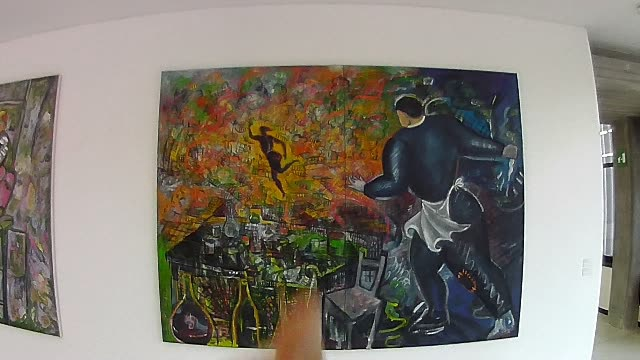
\includegraphics[width=0.2\linewidth]{Figures/like_16695_16718_all1.jpg}
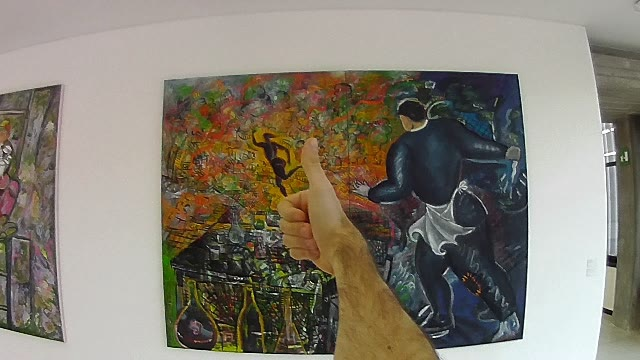
\includegraphics[width=0.2\linewidth]{Figures/like_16695_16718_all14.jpg}
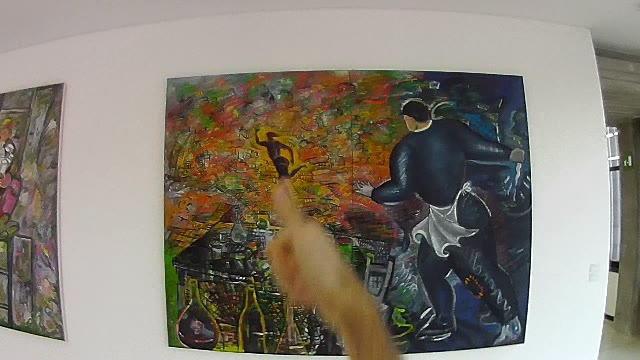
\includegraphics[width=0.2\linewidth]{Figures/like_16695_16718_all21.jpg}
}\\
\subfigure[\textit{Dislike} gesture]{
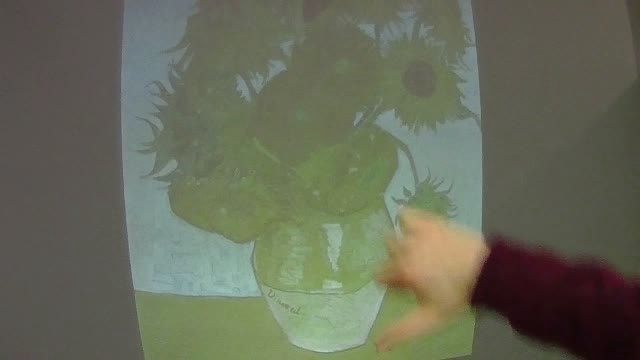
\includegraphics[width=0.2\linewidth]{Figures/dislike_10962_11000_all3.jpg}
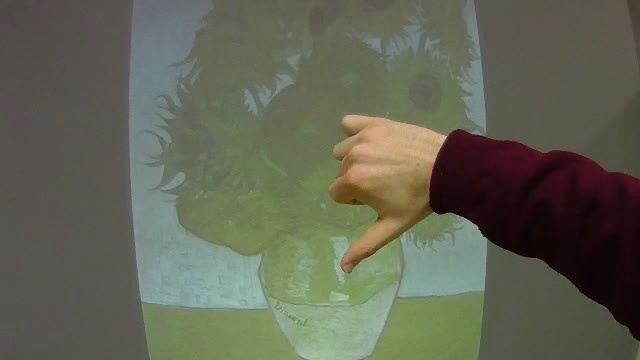
\includegraphics[width=0.2\linewidth]{Figures/dislike_10962_11000_all23.jpg}
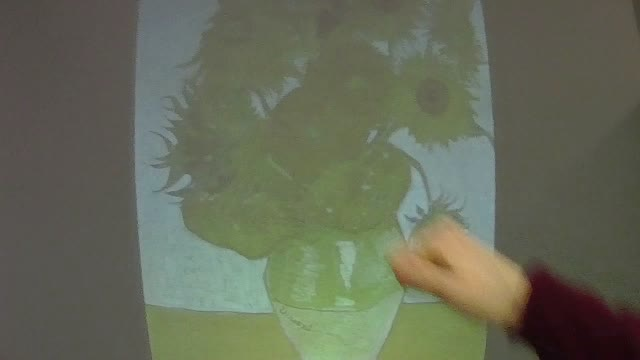
\includegraphics[width=0.2\linewidth]{Figures/dislike_10962_11000_all35.jpg}
}\\
\subfigure[\textit{Ok} gesture in the \textit{museum} setting, in low light]{
  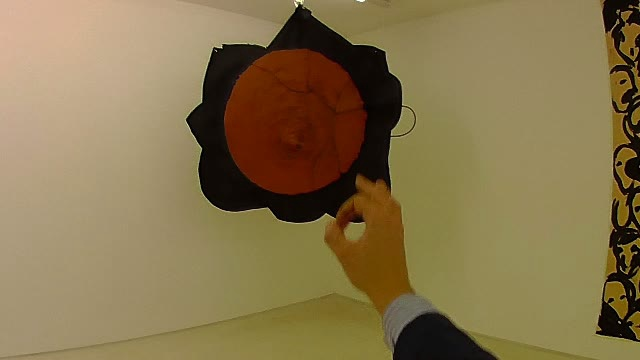
\includegraphics[width=0.2\linewidth]{Figures/ok_2696_2735_all5.jpg}
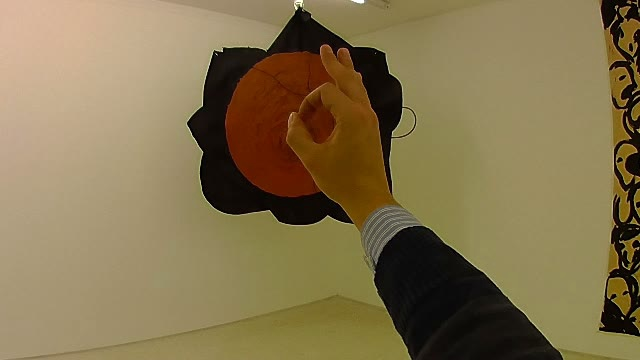
\includegraphics[width=0.2\linewidth]{Figures/ok_2696_2735_all23.jpg}
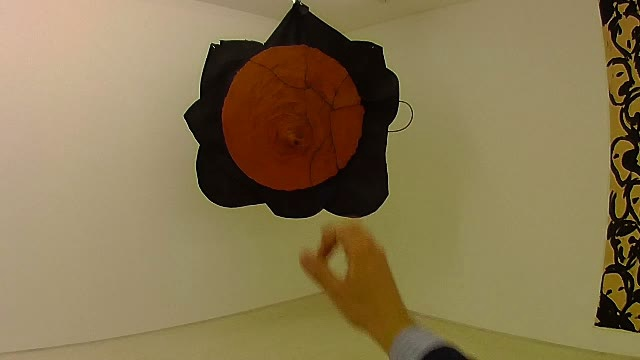
\includegraphics[width=0.2\linewidth]{Figures/ok_2696_2735_all36.jpg}
}\\
\subfigure[\textit{Point} gesture]{
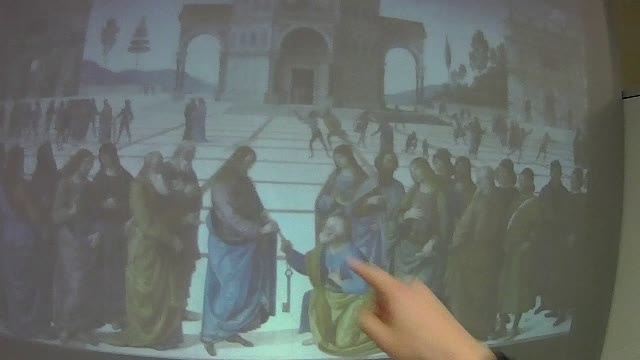
\includegraphics[width=0.2\linewidth]{Figures/point_4624_4654_all3.jpg}
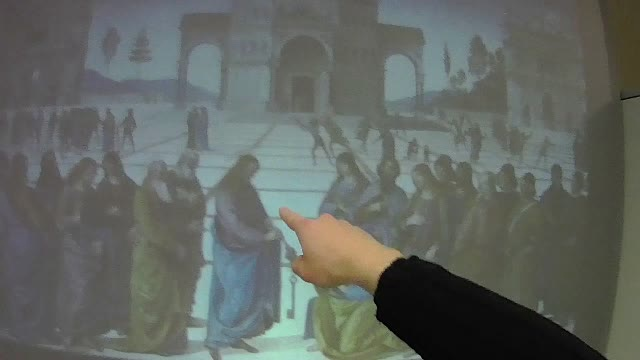
\includegraphics[width=0.2\linewidth]{Figures/point_4624_4654_all8.jpg}
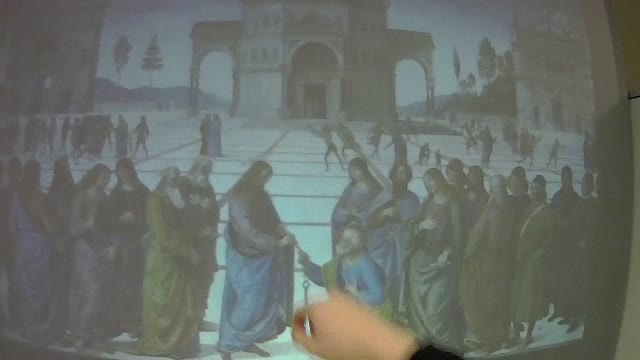
\includegraphics[width=0.2\linewidth]{Figures/point_4624_4654_all28.jpg}
}\\
\subfigure[\textit{Slide right to left} gesture in the \textit{museum} setting, while another visitor walks in]{
  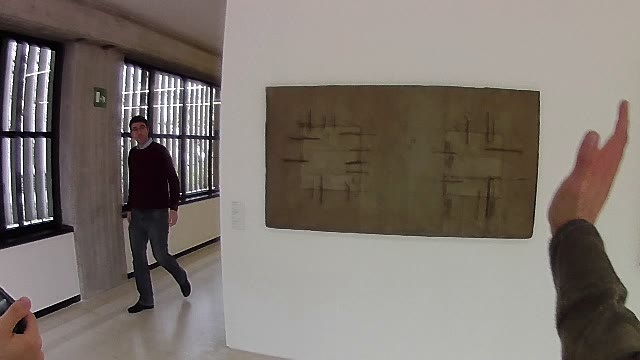
\includegraphics[width=0.2\linewidth]{Figures/slide_2_7348_7383_all12.jpg}
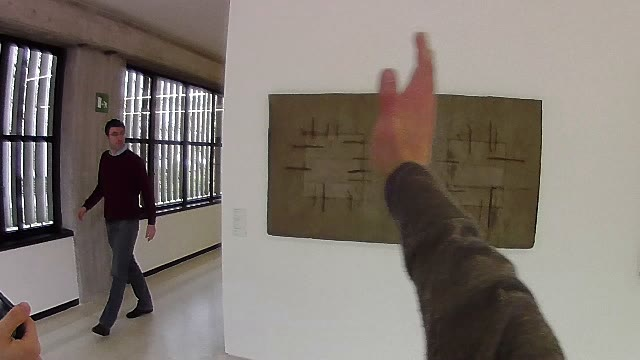
\includegraphics[width=0.2\linewidth]{Figures/slide_2_7348_7383_all20.jpg}
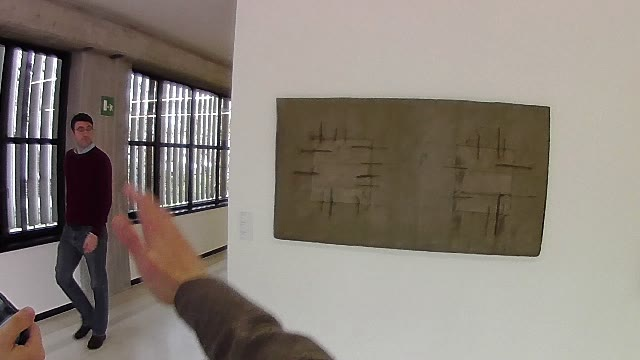
\includegraphics[width=0.2\linewidth]{Figures/slide_2_7348_7383_all30.jpg}
}\\
\subfigure[\textit{Slide left to right} gesture in the \textit{demo room} setting performed by user 3]{
  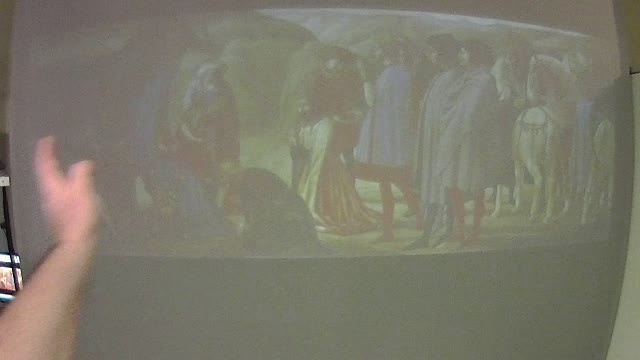
\includegraphics[width=0.2\linewidth]{Figures/slide_2_2030_2058_all7.jpg}
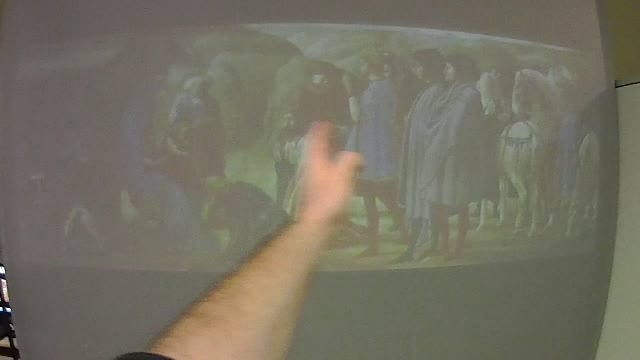
\includegraphics[width=0.2\linewidth]{Figures/slide_2_2030_2058_all14.jpg}
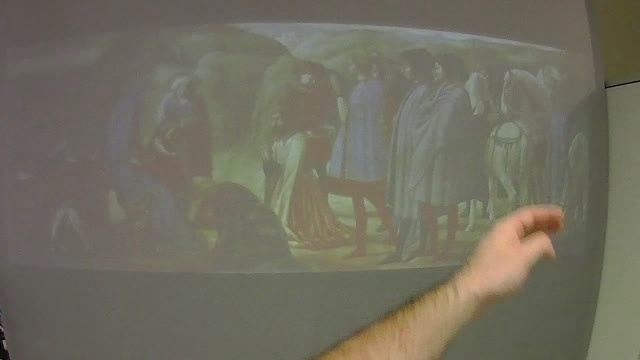
\includegraphics[width=0.2\linewidth]{Figures/slide_2_2030_2058_all23.jpg}
}\\
\subfigure[\textit{Take a picture} gesture in the \textit{demo room} setting]{
  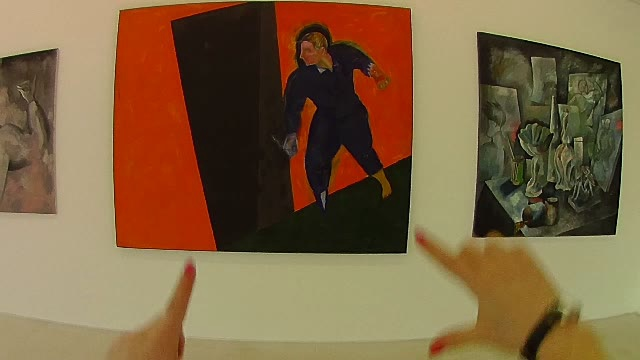
\includegraphics[width=0.2\linewidth]{Figures/take_a_picture_23956_24002_all2.jpg}
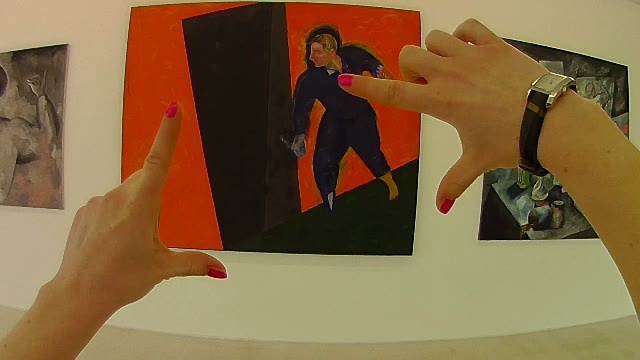
\includegraphics[width=0.2\linewidth]{Figures/take_a_picture_23956_24002_all25.jpg}
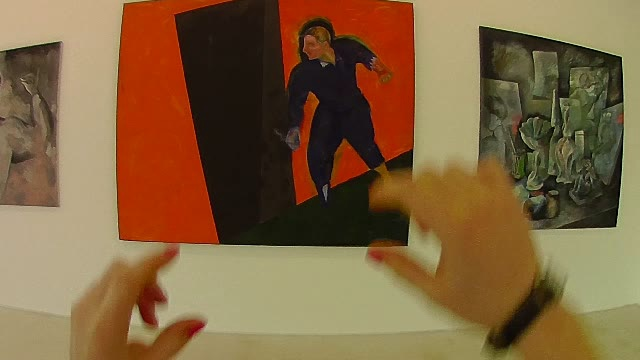
\includegraphics[width=0.2\linewidth]{Figures/take_a_picture_23956_24002_all43.jpg}
}
\caption{Sample gestures from the \datasetunimore{} dataset.}
\label{example-unimore}
\end{figure}

We then propose the \datasetunimore{} dataset, a gesture recognition dataset taken from the ego-centric perspective in a virtual museum environment. It consists of 700 video sequences, all shot with a wearable camera, in an interactive exhibition room, in which paintings and artworks are projected over a wall, in a virtual museum fashion (see figure \ref{example-unimore}). The camera is placed on the user's head and captures a 800 $\times$ 450, 25 frames per second 24-bit RGB image sequence. In this setting, five different users perform seven hand gestures: \textit{like}, \textit{dislike}, \textit{point}, \textit{ok}, \textit{slide left to right}, \textit{slide right to left} and \textit{take a picture}. Some of them (like the \textit{point}, \textit{ok}, \textit{like} and \textit{dislike} gestures) are statical, others (like the two \textit{slide} gestures) are dynamical. 
This dataset is very challenging since there is fast camera motion and users have not been trained before recording their gestures, so that each user performs the gestures in a slightly different way, as would happen in a realistic context. We have publicly released our dataset\footnote{\url{http://imagelab.ing.unimore.it/files/ego_virtualmuseum.zip}}.

%In the demo room setting, users perform gestures in front of a wall over which the works of art are projected. This setting is quite controlled: the illumination is constant, the art works are in low light, while hands are well illuminated. In the same way, in the \textit{museum} setting, users perform gestures in front of real artworks inside a museum. This is a realistic and very challenging environment: the illumination changes, other visitors are present and sometimes walk in. 
Since Ego Vision applications are highly interactive, their setup step must be fast (i.e. few positive examples can be acquired). Therefore, to evaluate the proposed gesture recognition approach, we train a 1-vs-1 linear classifier for each user using only two randomly chosen gestures per class as training set. The reported results are the average over 100 independent runs.

In Table \ref{gesture_comparison} we show the gesture recognition accuracy for each of the five subjects, and we also compare with the ones obtained without the use of the hand segmentation mask for camera motion removal and trajectories pruning.  Results show that our approach is well suited to recognize hand gestures in the ego-centric domain, even using only two positive samples per gesture, and that the use of the segmentation mask can improve recognition accuracy.


\begin{table}
\begin{center}
\renewcommand{\arraystretch}{1.3}
\centering
\begin{tabular}{|l|c|c|}
\hline
User							& No segmentation & With segmentation  \\
\hline
\hline
Subject 1				 			& 0.91 		& \textbf{0.95} \\
Subject 2			 				& 0.87 		& \textbf{0.87} \\
Subject 3					 		& 0.92		& \textbf{0.95}\\
Subject 4							& \textbf{0.96}	& 0.94 \\
Subject 5							& 0.91		& \textbf{0.96} \\
\hline
Average						&  0.91	& \textbf{0.93}  \\
\hline
\end{tabular}
\end{center}
\caption{Gesture recognition accuracy on the \datasetunimore{} dataset with and without hand segmentation.}
\label{gesture_comparison}
\end{table}